\chapter{Results and Analysis}

This chapter reports the quantitative results as partial validation of the system. The current repository calibration bundle is used as the primary source for the results in this revised thesis. The results validate static ball localisation, static joint-touch localisation, and qualitative dynamic tracking behaviour. They do not constitute full closed-loop validation with a moving human target and live autonomous firing.

\section{Intrinsic Calibration Results}

Intrinsic calibration was performed at 1280 $\times$ 720 resolution for all four cameras using the ChArUco auto-capture procedure. Approximately 30--40 valid frames per camera were collected, and frames with insufficient corner coverage were excluded before calibration.

The resulting reprojection errors are acceptable for a low-cost prototype, but they should not be interpreted as guaranteeing final 3D accuracy. In this system, small errors in the intrinsic model interact with extrinsic calibration, tag placement, and camera geometry. The final accuracy must therefore be judged from the ground-truth 3D evaluations rather than from reprojection error alone.

\section{Extrinsic Calibration Results}

Extrinsic calibration uses the 24-tag AprilTag wall grid and robust PnP optimisation. The current repository state stores the active calibration bundle in the \texttt{arena\_fixed} structure and binds it through a calibration manifest. This is important because several earlier extrinsic files remain in the repository for provenance; the revised thesis refers to the active fixed bundle and the corresponding ground-truth evaluation reports.

Visual overlay validation confirms that known tag corners reproject plausibly into the camera images. However, the quantitative results below show that the system still contains a systematic 3D bias. This is an important finding rather than a formatting issue: it means the perception pipeline is repeatable but calibration-limited.

\section{Ball Static Localisation Results}

Table~\ref{tab:5_1} reports the current raw static ball localisation metrics from the 36-point ground-truth evaluation.

\begin{table}[htbp]
\centering
\caption{Ball static localisation summary metrics, current raw evaluation}
\label{tab:5_1}
\begin{tabular}{|l|l|}
\hline
\textbf{Metric} & \textbf{Value} \\
\hline
Trials valid & 36 / 36 (100\%) \\
\hline
Mean 3D error & 156.90 mm \\
\hline
Median 3D error & 157.52 mm \\
\hline
RMSE & 172.05 mm \\
\hline
P90 & 236.38 mm \\
\hline
P95 & 288.34 mm \\
\hline
Maximum error & 361.83 mm \\
\hline
Mean reprojection error & 5.46 px \\
\hline
Mean cameras used & 2.74 \\
\hline
Mean detection ratio (hold window) & 1.000 \\
\hline
Mean temporal precision (std-norm) & 3.09 mm \\
\hline
P95 temporal precision & 11.62 mm \\
\hline
\end{tabular}
\end{table}

The static ball results show a clear distinction between repeatability and absolute accuracy. The mean temporal precision is 3.09 mm, indicating that repeated estimates of the same static point are highly stable during the hold window. However, the mean absolute error is 156.90 mm and the P95 is 288.34 mm. Therefore, the current raw system does not satisfy the original RQ1 target of mean error below 120 mm. This is a more conservative conclusion than the earlier corrected-pipeline framing and is better aligned with the current repository evaluation report.

\begin{figure}[htbp]
\centering
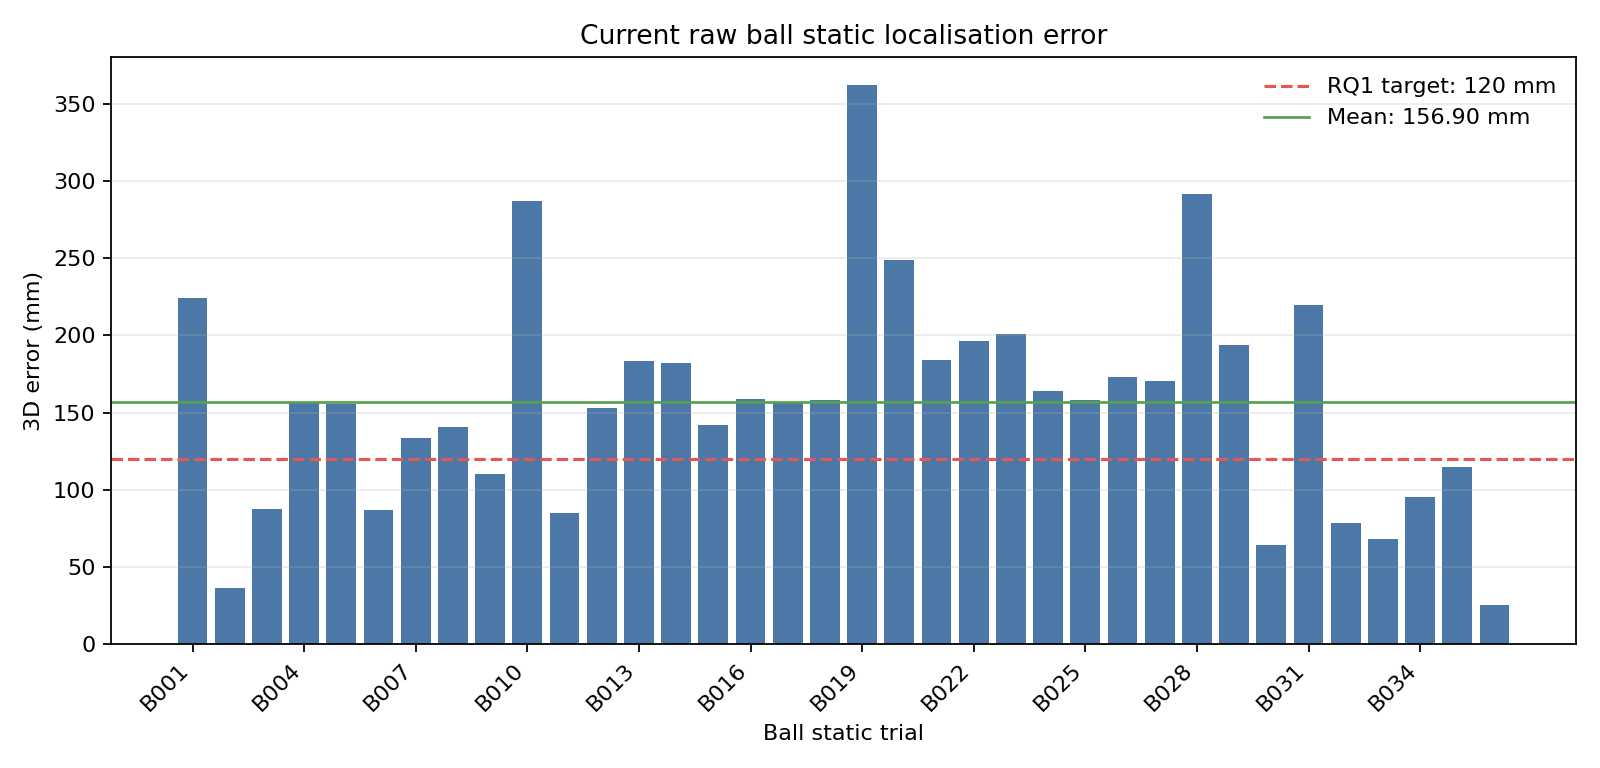
\includegraphics[width=0.9\textwidth]{figures/current_ball_error_by_trial}
\caption{Current raw ball static localisation error by trial. The distribution shows stable detection across all 36 trials but a substantial systematic error component.}
\label{fig:5_1}
\end{figure}

The dominant bias components are X = +60.22 mm, Y = +13.06 mm, and Z = \textminus{}104.34 mm. The negative Z bias is physically plausible because all cameras are mounted near the ceiling and observe low ball positions through shallow downward-looking rays. Small camera-height or pitch errors therefore propagate into vertical triangulation bias.

\begin{figure}[htbp]
\centering
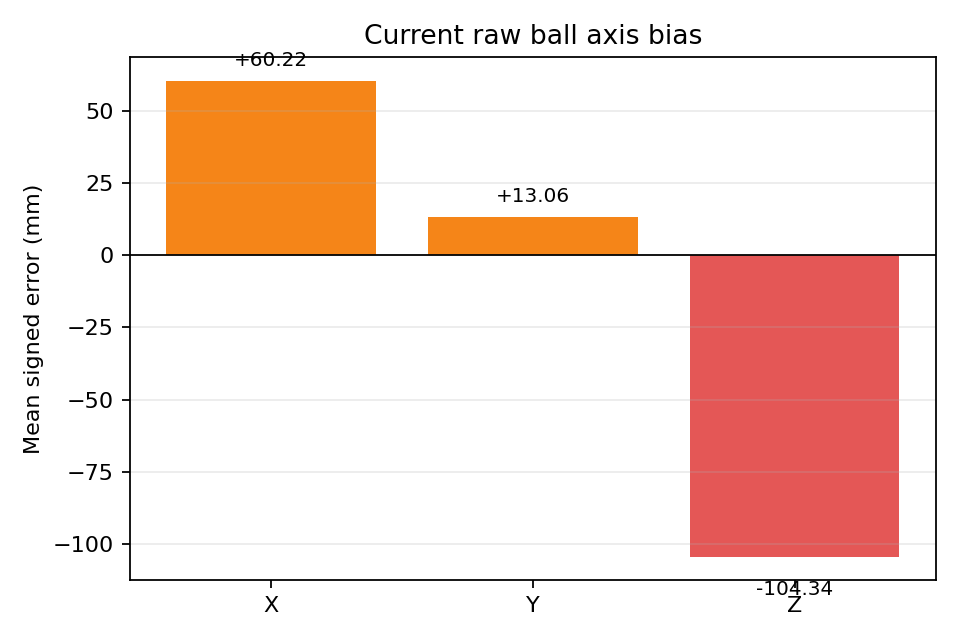
\includegraphics[width=0.75\textwidth]{figures/current_ball_axis_bias}
\caption{Current raw ball localisation axis bias. The largest component is the negative Z bias, consistent with the elevated camera geometry.}
\label{fig:5_2}
\end{figure}

The repository includes a linear correction model for this bias. Such a model is useful for runtime compensation and for diagnosing systematic calibration error. However, because the correction is fitted from ground-truth trials, corrected accuracy should not be treated as final performance unless it is evaluated on an independent held-out dataset. For this reason, the raw values in Table~\ref{tab:5_1} are used as the primary evidence in the revised thesis.

\section{Human Pose Joint-Touch Results}

Table~\ref{tab:5_2} reports the current joint-touch results. Of 81 planned trials, 62 are valid and 19 are missing or failed. The invalid trials are part of the result because they reflect real visibility and occlusion constraints in the camera setup.

\begin{table}[htbp]
\centering
\caption{Joint-touch 3D ground-truth summary metrics, current evaluation}
\label{tab:5_2}
\begin{tabular}{|l|l|}
\hline
\textbf{Metric} & \textbf{Value} \\
\hline
Trials valid & 62 / 81 (76.5\%) \\
\hline
Mean 3D error & 178.98 mm \\
\hline
Median 3D error & 181.17 mm \\
\hline
RMSE & 183.69 mm \\
\hline
P90 & 227.35 mm \\
\hline
P95 & 243.77 mm \\
\hline
Maximum error & 271.13 mm \\
\hline
Mean temporal precision (std-norm) & 4.39 mm \\
\hline
P95 temporal precision & 9.17 mm \\
\hline
\end{tabular}
\end{table}

The global mean joint error is 178.98 mm, which is just below the 180 mm target in RQ2. This result should be interpreted carefully. It supports the feasibility of the low-cost multi-camera joint-localisation approach for valid static holds, but the margin is narrow and the result excludes 19 invalid or missing trials. The P95 of 243.77 mm remains below the 280 mm global acceptance threshold defined for joint-touch evaluation.

\begin{table}[htbp]
\centering
\caption{Per-joint error breakdown, current evaluation}
\label{tab:5_3}
\begin{tabular}{|l|l|l|l|}
\hline
\textbf{Joint} & \textbf{Valid trials} & \textbf{Mean error (mm)} & \textbf{P95 (mm)} \\
\hline
right\_knee & 17 & 148.44 & 213.40 \\
\hline
right\_hip & 27 & 182.15 & 218.12 \\
\hline
left\_shoulder & 18 & 203.09 & 246.42 \\
\hline
\end{tabular}
\end{table}

The per-joint breakdown shows the expected hierarchy. The right knee has the lowest mean error because it is often visible from multiple views and lies in a favourable portion of the camera volume. The right hip has higher error because it is affected by torso occlusion and because the anatomical keypoint is harder to observe consistently. The left shoulder has the highest mean error, particularly because shoulder trials occur at greater heights and are more likely to be affected by self-occlusion and elevated-camera geometry.

\begin{figure}[htbp]
\centering
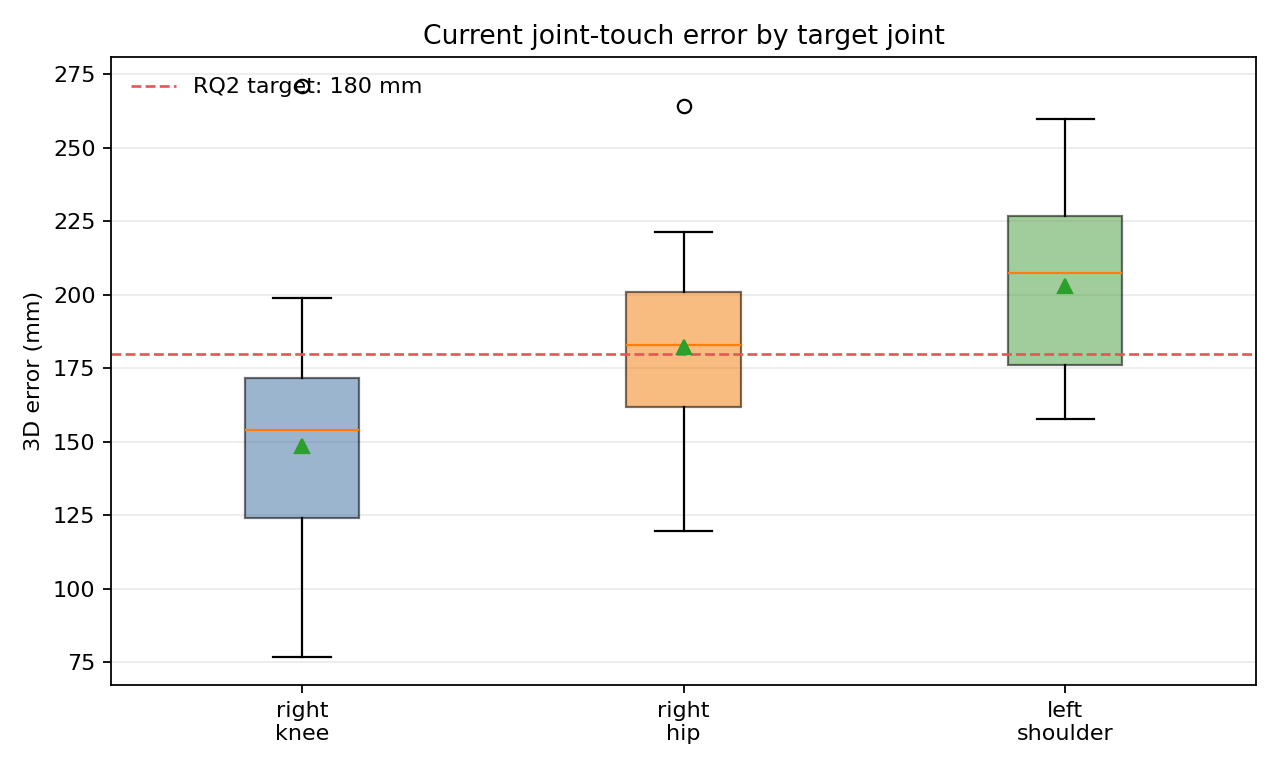
\includegraphics[width=0.82\textwidth]{figures/current_joint_error_by_joint}
\caption{Current joint-touch error distribution by target joint. Higher shoulder error reflects reduced visibility and stronger vertical-bias effects at greater heights.}
\label{fig:5_3}
\end{figure}

The mean temporal precision for valid joint holds is 4.39 mm, with a P95 precision of 9.17 mm. As with the ball results, this indicates that the pipeline is repeatable over short static windows. The dominant limitation is not random jitter but systematic spatial error and visibility failure. This distinction matters for future work: improving calibration and camera placement should reduce mean error, whereas increasing frame-level smoothing alone will not eliminate a fixed spatial bias.

\begin{figure}[htbp]
\centering
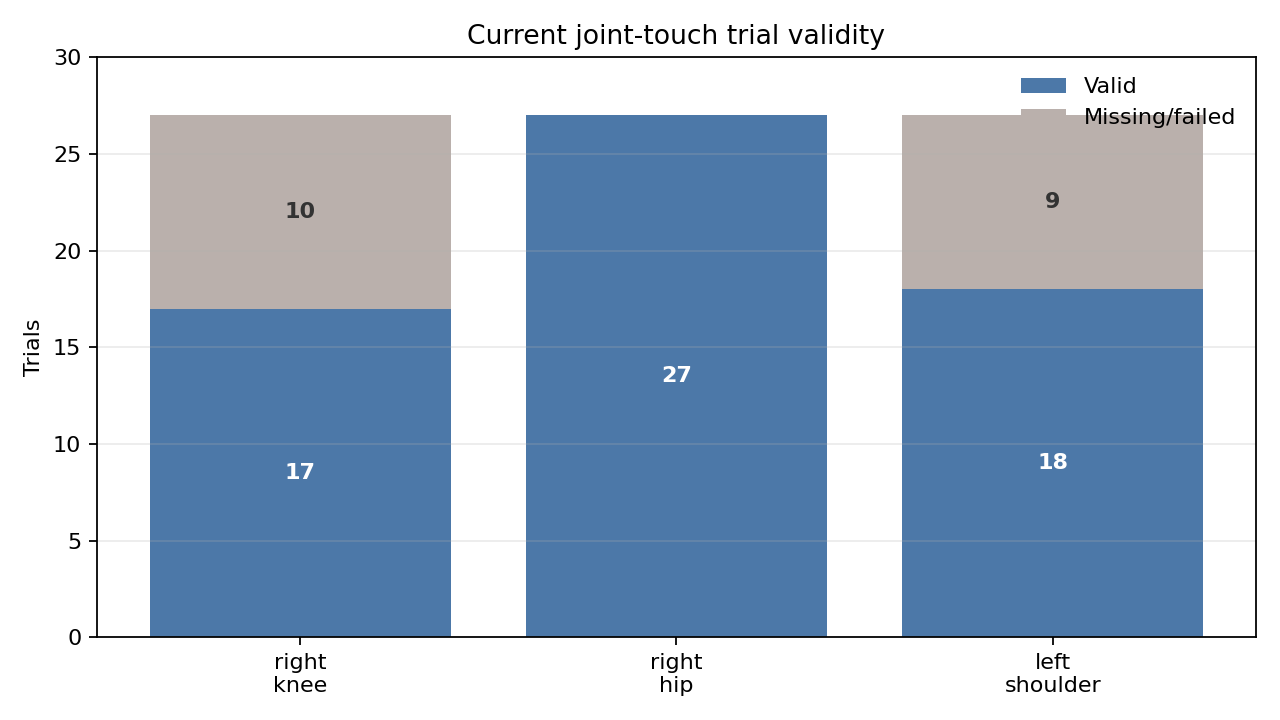
\includegraphics[width=0.82\textwidth]{figures/current_joint_validity_by_joint}
\caption{Valid and missing joint-touch trials by target joint in the current evaluation. Missing trials reveal visibility limitations that must be addressed before full closed-loop deployment.}
\label{fig:5_4}
\end{figure}

\section{Dynamic Detection Results}

\begin{figure}[htbp]
\centering
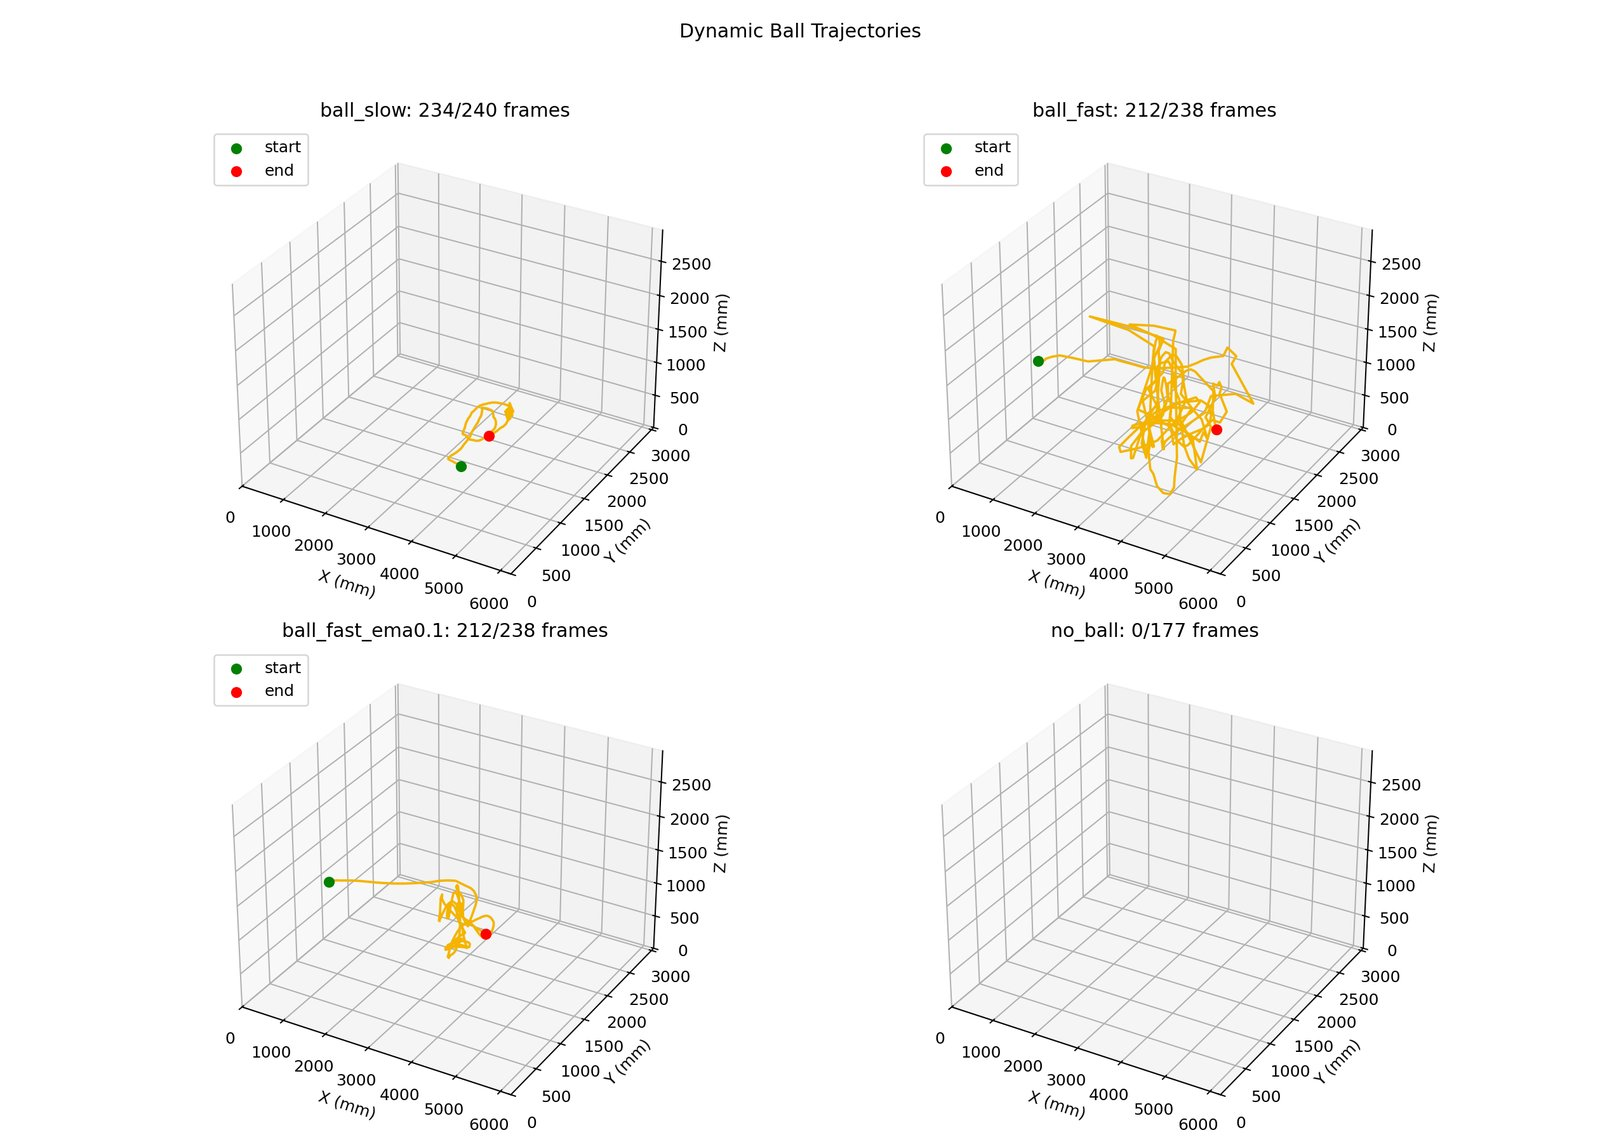
\includegraphics[width=0.8\textwidth]{figures/image5_9_dynamic}
\caption{Dynamic ball trajectory reconstructions from validation clips. These clips support qualitative tracking assessment but are not a substitute for closed-loop moving-target firing validation.}
\label{fig:5_5}
\end{figure}

The dynamic clips show that the system can maintain plausible 3D trajectories under moderate movement and can suppress short-term jitter with smoothing. The \textit{no\_ball} control clip is used to check that the detector does not produce sustained false trajectories when the ball is absent. The \textit{ball\_fast} clip is more challenging because motion blur and rapid acceleration reduce detection confidence and increase the likelihood of outliers.

These dynamic results are useful as stress tests of the tracking pipeline, but they are not a complete validation of the thesis's long-term goal. A complete demonstration would require an independently measured moving target, a fired ball, a recorded impact or interception point, and a comparison between intended and achieved target location. That experiment has not yet been completed. Therefore, the present results should be stated as partial validation: static localisation is quantified, dynamic tracking is qualitatively demonstrated, and closed-loop moving-target firing remains future work.
